% CVPR 2027 Paper Template; see https://github.com/cvpr-org/author-kit

\documentclass[10pt,twocolumn,letterpaper]{article}

%%%%%%%%% PAPER TYPE  - PLEASE UPDATE FOR FINAL VERSION
% \usepackage{cvpr}              % To produce the CAMERA-READY version
\usepackage[review]{cvpr}      % To produce the REVIEW version
% \usepackage[pagenumbers]{cvpr} % To force page numbers, e.g. for an arXiv version

% Import additional packages in the preamble file, before hyperref
%% This file contains a number of tweaks that are typically applied to the main document.
%% They are not enabled by default, but can be enabled by uncommenting the relevant lines.

%%
%% Inline annotations; for predefined colors, refer to "dvipsnames" in the xcolor package:
%% https://tinyurl.com/overleaf-colors
%%
\newcommand{\red}[1]{{\color{red}#1}}
\newcommand{\todo}[1]{{\color{red}#1}}
\newcommand{\TODO}[1]{\textbf{\color{red}[TODO: #1]}}
%%
%% disable for camera ready / submission by uncommenting these lines  
%%
% \renewcommand{\TODO}[1]{}
% \renewcommand{\todo}[1]{#1}

%%
%% work harder in optimizing text layout. Typically shrinks text by 1/6 of page, enable
%% it at the very end of the writing process, when you are just above the page limit
%%
% \usepackage{microtype}

%%
%% fine-tune paragraph spacing
%%
% \renewcommand{\paragraph}[1]{\vspace{.5em}\noindent\textbf{#1.}}

%%
%% globally adjusts space between figure and caption
%%
% \setlength{\abovecaptionskip}{.5em}


%%
%% Allows "the use of \paper to refer to the project name"
%% with automatic management of space at the end of the word
%%
% \usepackage{xspace}
% \newcommand{\paper}{ProjectName\xspace}

%%
%% Commonly used math definitions
%%
% \DeclareMathOperator*{\argmin}{arg\,min}
% \DeclareMathOperator*{\argmax}{arg\,max}

%%
%% Tigthen underline
%%
% \usepackage{soul}
% \setuldepth{foobar}
\usepackage{booktabs}
\usepackage{amssymb}
\usepackage{amsmath,amsfonts}
\usepackage{array}
\usepackage{tabularx}

% It is strongly recommended to use hyperref, especially for the review version.
% hyperref with option pagebackref eases the reviewers' job.
% Please disable hyperref *only* if you encounter grave issues, 
% e.g. with the file validation for the camera-ready version.
%
% If you comment hyperref and then uncomment it, you should delete *.aux before re-running LaTeX.
% (Or just hit 'q' on the first LaTeX run, let it finish, and you should be clear).
\definecolor{cvprblue}{rgb}{0.21,0.49,0.74}
\usepackage[pagebackref,breaklinks,colorlinks,allcolors=cvprblue]{hyperref}

\def\confName{CVPR}
\def\confYear{2027}

%%%%%%%%% TITLE - PLEASE UPDATE
\title{Learning from Filter-Corrected Labels: Reducing Annotation Costs via the Filtering Mechanism}

%%%%%%%%% AUTHORS - PLEASE UPDATE
\author{
    Anonymous Submission
}
% \author{First Author\\
% Institution1\\
% Institution1 address\\
% {\tt\small firstauthor@i1.org}
% % For a paper whose authors are all at the same institution,
% % omit the following lines up until the closing ``}''.
% % Additional authors and addresses can be added with ``\and'',
% % just like the second author.
% % To save space, use either the email address or home page, not both
% \and
% Second Author\\
% Institution2\\
% First line of institution2 address\\
% {\tt\small secondauthor@i2.org}
% }

\begin{document}
\maketitle
% \begin{abstract}
The ABSTRACT is to be in fully justified italicized text, at the top of the left-hand column, below the author and affiliation information.
Use the word ``Abstract'' as the title, in 12-point Times, boldface type, centered relative to the column, initially capitalized.
The abstract is to be in 10-point, single-spaced type.
Leave two blank lines after the Abstract, then begin the main text.
Look at previous \confName abstracts to get a feel for style and length.
\end{abstract}    
% \section{Introduction}
\label{sec:intro}

Please follow the steps outlined below when submitting your manuscript to the IEEE Computer Society Press.
This style guide now has several important modifications (for example, you are no longer warned against the use of sticky tape to attach your artwork to the paper), so all authors should read this new version.

%-------------------------------------------------------------------------
\subsection{Language}

All manuscripts must be in English.

\subsection{Dual submission}

Please refer to the author guidelines on the \confName\ \confYear\ web page for a
discussion of the policy on dual submissions.

\subsection{Paper length}
Papers, excluding the references section, must be no longer than eight pages in length.
The references section will not be included in the page count, and there is no limit on the length of the references section.
For example, a paper of eight pages with two pages of references would have a total length of 10 pages.
{\bf There will be no extra page charges for \confName\ \confYear.}

Overlength papers will simply not be reviewed.
This includes papers where margins and formatting are deemed to have been significantly altered from those laid down by this style guide.
Note that this \LaTeX\ guide already sets the figure captions and references in a smaller font.
The reason why such papers will not be reviewed is that there is no provision for supervised revisions of manuscripts.
The review process cannot determine the suitability of the paper for presentation in eight pages if it is reviewed in 11 pages.

%-------------------------------------------------------------------------
\subsection{The ruler}
The \LaTeX\ style defines a printed ruler that should be present in the version submitted for review.
The ruler is provided in order that reviewers may comment on particular lines in the paper without circumlocution.
If you are preparing a document using a non-\LaTeX\ document preparation system, arrange for an equivalent ruler to appear on the final output pages.
The presence or absence of the ruler should not change the appearance of any other content on the page.
The camera-ready copy should not contain a ruler.
(\LaTeX\ users may use the options of \texttt{cvpr.sty} to switch between different versions.)

Reviewers:
note that the ruler measurements do not align well with lines in the paper --- this turns out to be very difficult to do well when the paper contains many figures and equations, and, when done, looks ugly.
Use fractional references (\eg, this line is $087.5$), although in most cases the approximate location would be adequate.



\subsection{Mathematics}

Please, number all of your sections and displayed equations as in these examples:
\begin{equation}
  E = m\cdot c^2
  \label{eq:important}
\end{equation}
and
\begin{equation}
  v = a\cdot t.
  \label{eq:also-important}
\end{equation}
It is important for the reader to be able to refer to any particular equation.
Just because you did not refer to it in the text does not mean that some future reader might not need to refer to it.
It is cumbersome to have to use circumlocutions like ``the equation second from the top of page 3 column 1''.
(Note that the ruler will not be present in the final copy, so is not an alternative to equation numbers).
All authors will benefit from reading Mermin's description of how to write mathematics:
\url{http://www.pamitc.org/documents/mermin.pdf}.

\subsection{Blind review}

Many authors misunderstand the concept of anonymizing for blind review.
Blind review does not mean that one must remove citations to one's own work---in fact it is often impossible to review a paper unless the previous citations are known and available.

Blind review means that you do not use the words ``my'' or ``our'' when citing previous work.
That is all.
(But see below for tech reports.)

Saying ``this builds on the work of Lucy Smith [1]'' does not mean that you are Lucy Smith;
it says that you are building on her work.
If you are Smith and Jones, do not say ``as we show in [7]'', say ``as Smith and Jones show in [7]'' and at the end of the paper, include reference 7 as you would any other cited work.

An example of a bad paper just asking to be rejected:
\begin{quote}
\begin{center}
    An analysis of the frobnicatable foo filter.
\end{center}

   In this paper, we present a performance analysis of our previous paper [1], and show that it is inferior to all previously known methods.
   Why the previous paper was accepted without this analysis is beyond me.

   [1] Removed for blind review
\end{quote}


An example of an acceptable paper:
\begin{quote}
\begin{center}
     An analysis of the frobnicatable foo filter.
\end{center}

   In this paper, we present a performance analysis of the paper of Smith \etal [1], and show it to be inferior to all previously known methods.
   Why the previous paper was accepted without this analysis is beyond me.

   [1] Smith, L and Jones, C. ``The frobnicatable foo filter, a fundamental contribution to human knowledge''. Nature 381(12), 1-213.
\end{quote}

If you are making a submission to another conference at the same time that covers similar or overlapping material, you may need to refer to that submission to explain the differences, just as you would if you had previously published related work.
In such cases, include the anonymized parallel submission~\cite{Authors14} as supplemental material and cite it as
\begin{quote}
[1] Authors. ``The frobnicatable foo filter'', F\&G 2014 Submission ID 324, Supplied as supplemental material {\tt fg324.pdf}.
\end{quote}

Finally, you may feel you need to tell the reader that more details can be found elsewhere and refer them to a technical report.
For conference submissions, the paper must stand on its own, and not {\em require} the reviewer to go to a tech report for further details.
Thus, you may say in the body of the paper ``further details may be found in~\cite{Authors14b}''.
Then submit the tech report as supplemental material.
Again, do not assume that the reviewers will read this material.

Sometimes your paper is about a problem that you tested using a tool that is widely known to be restricted to a single institution.
For example, let's say it's 1969, you have solved a key problem on the Apollo lander, and you believe that the 1970 audience would like to hear about your
solution.
The work is a development of your celebrated 1968 paper entitled ``Zero-g frobnication: How being the only people in the world with access to the Apollo lander source code makes us a wow at parties'', by Zeus \etal.

You can handle this paper like any other.
Do not write ``We show how to improve our previous work [Anonymous, 1968].
This time we tested the algorithm on a lunar lander [name of lander removed for blind review]''.
That would be silly, and would immediately identify the authors.
Instead write the following:
\begin{quotation}
\noindent
   We describe a system for zero-g frobnication.
   This system is new because it handles the following cases:
   A, B.  Previous systems [Zeus et al. 1968] did not  handle case B properly.
   Ours handles it by including a foo term in the bar integral.

   ...

   The proposed system was integrated with the Apollo lunar lander, and went all the way to the moon, don't you know.
   It displayed the following behaviours, which show how well we solved cases A and B: ...
\end{quotation}
As you can see, the above text follows standard scientific convention, reads better than the first version, and does not explicitly name you as the authors.
A reviewer might think that it is likely that the new article was written by Zeus \etal, but cannot make any decision based on that guess.
He or she would have to be sure that no other authors could have been contracted to solve problem B.
\medskip

\noindent
FAQ\medskip\\
{\bf Q:} Are acknowledgements OK?\\
{\bf A:} No.  Leave them for the final copy.\medskip\\
{\bf Q:} How do I cite my results reported in open challenges?
{\bf A:} To conform with the double-blind review policy, you can report results of other challenge participants together with your results in your paper.
However, for your results, you should not identify yourself and should not mention your participation in the challenge.
Instead, present your results referring to the method proposed in your paper and draw conclusions based on the experimental comparison with other results.\medskip\\

\begin{figure}[t]
  \centering
  \fbox{\rule{0pt}{2in} \rule{0.9\linewidth}{0pt}}
   %\includegraphics[width=0.8\linewidth]{egfigure.eps}

   \caption{Example of caption.
   It is set in Roman so that mathematics (always set in Roman: $B \sin A = A \sin B$) may be included without an ugly clash.}
   \label{fig:onecol}
\end{figure}

\subsection{Miscellaneous}

\noindent
Compare the following:\\
\begin{tabular}{ll}
 \verb'$conf_a$' &  $conf_a$ \\
 \verb'$\mathit{conf}_a$' & $\mathit{conf}_a$
\end{tabular}\\
See The \TeX book, p165.

The space after \eg, meaning ``for example'', should not be a sentence-ending space.
So \eg is correct, {\em e.g.} is not.
The provided \verb'\eg' macro takes care of this.

When citing a multi-author paper, you may save space by using ``et alia'', shortened to ``\etal'' (not ``{\em et.\ al.}'' as ``{\em et}'' is a complete word).
If you use the \verb'\etal' macro provided, then you need not worry about double periods when used at the end of a sentence as in Alpher \etal.
However, use it only when there are three or more authors.
Thus, the following is correct:
   ``Frobnication has been trendy lately.
   It was introduced by Alpher~\cite{Alpher02}, and subsequently developed by
   Alpher and Fotheringham-Smythe~\cite{Alpher03}, and Alpher \etal~\cite{Alpher04}.''

This is incorrect: ``... subsequently developed by Alpher \etal~\cite{Alpher03} ...'' because reference~\cite{Alpher03} has only two authors.

\begin{figure*}
  \centering
  \begin{subfigure}{0.68\linewidth}
    \fbox{\rule{0pt}{2in} \rule{.9\linewidth}{0pt}}
    \caption{An example of a subfigure.}
    \label{fig:short-a}
  \end{subfigure}
  \hfill
  \begin{subfigure}{0.28\linewidth}
    \fbox{\rule{0pt}{2in} \rule{.9\linewidth}{0pt}}
    \caption{Another example of a subfigure.}
    \label{fig:short-b}
  \end{subfigure}
  \caption{Example of a short caption, which should be centered.}
  \label{fig:short}
\end{figure*}

% \section{Formatting your paper}
\label{sec:formatting}

All text must be in two-column format.
The total allowable size of the text area is $6\frac78$ inches (17.46 cm) wide by $8\frac78$ inches (22.54 cm) high.
The columns should be $3\frac14$ inches (8.25 cm) wide, with a $\frac{5}{16}$ inch (0.8 cm) space between them.
The main title (on the first page) should begin 1 inch (2.54 cm) from the top edge of the page.
The second and following pages should begin 1 inch (2.54 cm) from the top edge.
On all pages, the bottom margin should be $1\frac{1}{8}$ inches (2.86 cm) from the bottom edge of the page for $8.5 \times 11$-inch paper;
for A4 paper, approximately $1\frac{5}{8}$ inches (4.13 cm) from the bottom edge of the
page.

%-------------------------------------------------------------------------
\subsection{Margins and page numbering}

All printed material, including text, illustrations, and charts, must be kept
within a print area $6\frac{7}{8}$ inches (17.46 cm) wide by $8\frac{7}{8}$ inches (22.54 cm)
high.
%
Page numbers should be in the footer, centered, and $\frac{3}{4}$ inches from the bottom of the page.
The review version should have page numbers, yet the final version submitted as camera ready should not show any page numbers.
The \LaTeX\ template takes care of this when used properly.



%-------------------------------------------------------------------------
\subsection{Type style and fonts}

Wherever Times is specified, Times Roman may also be used.
If neither is available on your word processor, please use the font closest in
appearance to Times to which you have access.

MAIN TITLE.
Center the title $1\frac{3}{8}$ inches (3.49 cm) from the top edge of the first page.
The title should be in Times 14-point, boldface type.
Capitalize the first letter of nouns, pronouns, verbs, adjectives, and adverbs;
do not capitalize articles, coordinate conjunctions, or prepositions (unless the title begins with such a word).
Leave two blank lines after the title.

AUTHOR NAME(s) and AFFILIATION(s) are to be centered beneath the title
and printed in Times 12-point, non-boldface type.
This information is to be followed by two blank lines.

The ABSTRACT and MAIN TEXT are to be in a two-column format.

MAIN TEXT.
Type main text in 10-point Times, single-spaced.
Do NOT use double-spacing.
All paragraphs should be indented 1 pica (approx.~$\frac{1}{6}$ inch or 0.422 cm).
Make sure your text is fully justified---that is, flush left and flush right.
Please do not place any additional blank lines between paragraphs.

The captions of the figures and tables should be in 9-point Roman type as in \cref{fig:onecol,fig:short}.
Short captions should be centered.  Table captions should be above tables, while figure captions should be below figures.

\noindent Callouts should be 9-point Helvetica, non-boldface type.
Initially capitalize only the first word of section titles and first-, second-, and third-order headings.

FIRST-ORDER HEADINGS.
(For example, {\large \bf 1. Introduction}) should be Times 12-point boldface, initially capitalized, flush left, with one blank line before and one blank line after.

SECOND-ORDER HEADINGS.
(For example, { \bf 1.1. Database elements}) should be Times 11-point boldface, initially capitalized, flush left, with one blank line before and one after.
If you require a third-order heading (we discourage it), use 10-point Times, boldface, initially capitalized, flush left, preceded by one blank line, followed by a period, and your text on the same line.

%-------------------------------------------------------------------------
\subsection{Footnotes}

Please use the footnotes\footnote{This is what a footnote looks like.
It often distracts the reader from the main flow of the argument.} sparingly.
Indeed, try to avoid footnotes altogether and include necessary peripheral observations in the text (within parentheses, if you prefer, as in this sentence).
If you wish to use a footnote, place it at the bottom of the column on the page on which it is referenced.
Use Times 8-point type, single-spaced.


%-------------------------------------------------------------------------
\subsection{Cross-references}

For the benefit of author(s) and readers, please use the
{\small\begin{verbatim}
  \cref{...}
\end{verbatim}}  command for cross-referencing to figures, tables, equations, or sections.
This will automatically insert the appropriate label alongside the cross-reference as in this example:
\begin{quotation}
  To see how our method outperforms previous work, see \cref{fig:onecol} and \cref{tab:example}.
  It is also possible to refer to multiple targets as once, \eg~to \cref{fig:onecol,fig:short-a}.
  You may also return to \cref{sec:formatting} or look at \cref{eq:also-important}.
\end{quotation}
If you do not wish to abbreviate the label, for example, at the beginning of the sentence, you can use
{\small\begin{verbatim}
  \Cref{...}
\end{verbatim}}
command. Here is an example:
\begin{quotation}
  \Cref{fig:onecol} is also quite important.
\end{quotation}

%-------------------------------------------------------------------------
\subsection{References}

List and number all bibliographical references in 9-point Times, single-spaced, at the end of your paper.
When referenced in the text, include the citation number in square brackets, for
example~\cite{Authors14}.
Where appropriate, include page numbers and the name(s) of editors of referenced books.
When citing multiple papers at once, make sure that you cite them in numerical order such as this \cite{Alpher02,Alpher03,Alpher05,Authors14b,Authors14}.
If you use the template as advised, this will be taken care of automatically.

\begin{table}
  \caption{Results.   Ours is better.}
  \label{tab:example}
  \centering
  \begin{tabular}{@{}lc@{}}
    \toprule
    Method & Frobnability \\
    \midrule
    Theirs & Frumpy \\
    Yours & Frobbly \\
    Ours & Makes one's heart Frob\\
    \bottomrule
  \end{tabular}
\end{table}

%-------------------------------------------------------------------------
\subsection{Illustrations, graphs, and photographs}

All graphics should be centered.
In \LaTeX, avoid using the \texttt{center} environment for this purpose, as this adds potentially unwanted whitespace.
Instead, use
{\small\begin{verbatim}
  \centering
\end{verbatim}}
at the beginning of your figure.
Please ensure that any point you wish to make is resolvable in a printed copy of the paper.
Resize fonts in figures to match the font in the body text, and choose line widths that render effectively in print.
Readers (and reviewers), even of an electronic copy, may choose to print your paper in order to read it.
You cannot insist that they do otherwise and, therefore, must not assume that they can zoom in to see tiny details on a graphic.

When placing figures in \LaTeX, it is almost always best to use \verb+\includegraphics+, and to specify the figure width as a multiple of the line width as in the example below
{\small\begin{verbatim}
   \usepackage{graphicx} ...
   \includegraphics[width=0.8\linewidth]
                   {myfile.pdf}
\end{verbatim}
}


%-------------------------------------------------------------------------
\subsection{Color}

Please refer to the author guidelines on the \confName\ \confYear\ web page for a discussion of the use of color in your document.

If you use color in your plots, please keep in mind that a significant subset of reviewers and readers may have a color vision deficiency; red-green blindness is the most frequent kind.
Hence, avoid relying only on color as the discriminative feature in plots (such as red \vs green lines), but add a second discriminative feature to ease disambiguation.
% \section{Final copy}

You must include your signed IEEE copyright release form when you submit your finished paper.
We MUST have this form before your paper can be published in the proceedings.

Please direct any questions to the production editor in charge of these proceedings at the IEEE Computer Society Press:
\url{https://www.computer.org/about/contact}.

\begin{abstract}
Vision-language models provide inexpensive image labels, but correcting their errors under a limited annotation budget remains challenging. We study Filter-Corrected Labels (FCL-C), a protocol that selects distant instances within each pseudo-labeled class for correction using frozen CLIP features. The resulting data contain corrected labels and residual noisy annotations with different reliability. We combine cross-entropy on corrected instances with an AUC-based consistency objective on uncorrected instances. Its soft pair weights combine fixed CLIP probabilities with detached classifier predictions, retaining information beyond hard pseudo-labels. On five image-classification benchmarks, FCL improves accuracy over the compared weakly supervised implementations using a nominal correction rate of $30\%$. Additional controls examine prototype selection, the training objective, feature extractors, and synthetic errors in corrected labels. Correction is simulated using benchmark labels; the budget measures queried training labels rather than observed human annotation time.
\end{abstract}

\section{Introduction}\label{sec:intro}
Recent progress in Vision-Language Models (VLMs) has shown that they perform strongly on annotation tasks by aligning image and text representations \cite{radford2021clip}. These pre-trained models can assign labels to images without any task specific training. Large-scale image--text datasets further demonstrate the usefulness of weakly supervised visual representations \cite{gadre2023datacomp, schuhmann2022laion5b}.

However, labels produced by VLMs are often noisy and may degrade the overall quality of the annotated dataset. Models can confuse visually similar categories due to limited visual granularity or prompt sensitivity. As shown in Figure~\ref{fig:overview}(a), the model assigns ``Water Lily'' the highest confidence although the ground truth is ``Lotus''. To mitigate such noise, existing methods typically add verification stages to VLMs generated annotations. Examples include human verification of model generated labels \cite{wang2024humanllm}, collaborative systems that integrate human feedback to refine machine suggestions \cite{kim2024meganno}, and weak supervision frameworks that verify noisy programmatic labels before producing the final supervision \cite{ratner2017snorkel}.

Some annotation systems introduce additional modeling or iterative review stages, as illustrated in Figure~\ref{fig:overview}(b). For example, Snorkel \cite{ratner2016dataprog, ratner2017snorkel} constructs multiple heuristic labeling functions and applies generative modeling to estimate their accuracies before producing aggregated labels. ActiveAED \cite{weber2023activeaed} trains an auxiliary error detection model that repeatedly flags suspicious annotations for human review. These stages motivate a complementary approach that reuses frozen visual features for a single round of correction selection.

To address this limitation, we study a budgeted correction protocol called Filter-Corrected Labels (FCL-C), which uses a simple yet effective prototype to turn VLM predictions into high-quality labels with little human effort. The setting consists of low cost label verification based on prototype computation and distance based filtering, followed by human correction. Concretely, the VLM provides pseudo-labels first. For each candidate class, we then compute a class prototype by averaging the feature representations of its instances, forming a compact data center for that class. The distance between each instance and its class prototype defines a filter area that identifies instances requiring human correction. For example, as illustrated in Figure~\ref{fig:overview}(b), instances located in the yellow filter area are manually corrected. The selection step requires class means and within-class distances, without training an auxiliary detector. The resulting partition also defines which samples receive supervised classification loss and which receive a soft pairwise objective. 

In this paper, we further introduce an AUC-based consistency objective (AUC-C). AUC-C assigns soft pairwise weights to uncorrected instances using CLIP probabilities and detached classifier predictions. It combines these probabilities with the classifier posterior to obtain class dependent soft pair weights. In this way, AUC optimization can be extended to samples without reliable labels while retaining useful information from the uncorrected subset. For corrected instances, AUC-C uses a standard multiclass risk to anchor classifier learning. Experiments across diverse datasets confirm the effectiveness of the method.

\begin{figure*}[t] 
  \centering
  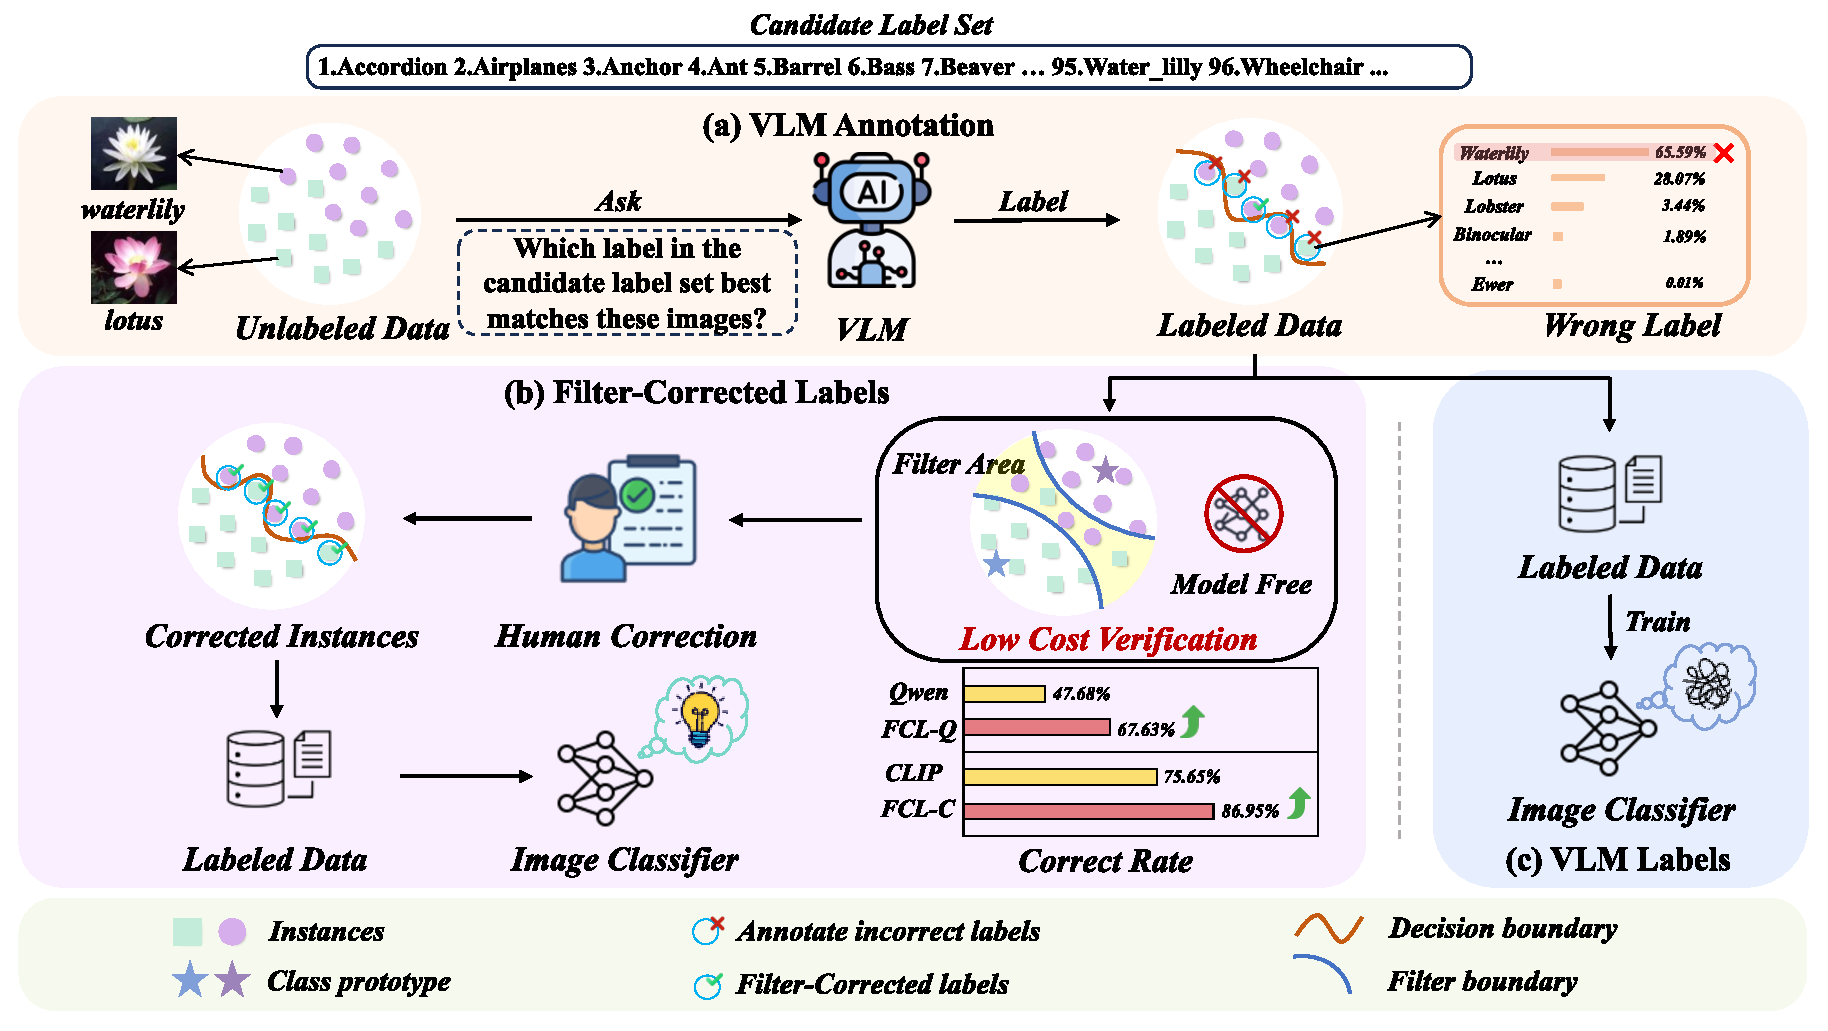
\includegraphics[width=0.9\textwidth]{./Figures/overview.pdf}
  \caption{Comparison between training with VLM-generated labels and training with Filter-Corrected Labels. CLIP ViT-L/14 supplies the zero-shot labels and frozen image features. Example images and categories are taken from the Caltech-101 dataset. FCL deploys human correction only for filtered instances, allocating the correction budget to selected annotations.}
  \label{fig:overview}
\end{figure*}

\begin{itemize}
    \item We study one-shot prototype-based correction of CLIP labels under a fixed query budget, separating corrected and uncorrected supervision through a shared selection mask.
    \item We combine corrected-sample cross-entropy with posterior-weighted pairwise learning on uncorrected instances. The pair weights interpolate between a fixed CLIP prior and detached classifier predictions.
    \item Experiments on five benchmarks compare classification accuracy, selection and loss controls, and sensitivity to synthetic correction errors under frozen-feature training.
\end{itemize}

\section{Related Work}
FCL draws on collaborative annotation, label correction, and pairwise learning.
\subsection{Collaborative Annotation}
Human–Model Collaborative Annotation reduces labeling cost by pairing model predictions with human verification \cite{papadopoulos2017extreme, maninis2018dextr, acuna2018polyrnnpp}. For example, programmatic approaches such as Snorkel \cite{ratner2016dataprog, ratner2017snorkel} showcased scalable weak supervision by aggregating heuristic labeling functions, reducing the need for manual annotation. More recently, Human–LLM Collaborative Annotation \cite{wang2024humanllm} shows that combining large language model predictions with selective human verification can reduce annotation cost while maintaining accuracy. MEGAnno+ \cite{kim2024meganno} reports improved annotation throughput through structured human–model interaction.

Our work investigates Human--VLM Collaborative Annotation (HVCA), using VLM labels to derive class prototypes without training an additional selection model. We utilize the prototypes to define a filter area that flags instances needing correction, enabling a simple and effective HVCA method.

\subsection{Weakly Supervised Learning}
Weakly supervised learning trains models from incomplete or inaccurate annotations, and this work is  primarily connected to noisy labels learning. Noisy labels learning assumes corrupted supervision and aims to reduce the impact of incorrect labels through sample selection, relabeling, or robust training objectives. Representative methods are Co-Teaching \cite{han2018coteaching}, DivideMix \cite{li2020dividemix}, early learning regularization \cite{liu2020elr}, JoCoR \cite{wei2020jocor}, error bounded correction \cite{zheng2020ebc, song2023noisysurvey}, and confident learning \cite{northcutt2021cl}.

Noisy-label learning can use either human or machine annotations. FCL is also closely related to hybrid human-machine labeling and active label cleaning. Active Learning typically employs iterative sampling strategies to select the most informative instances for human annotation to reduce total labeling effort \cite{jan2014active, qiu2023mcal}. Iterative AL updates the selection strategy as labels become available. In contrast, our FCL-C setting leverages the pre-trained knowledge of Vision-Language Models (VLMs) as a strong prior. It utilizes a simple yet effective prototype-based filter to isolate noisy regions for targeted human correction, without training an auxiliary selection network. Furthermore, we propose an AUC-based consistency objective on the remaining uncorrected instances to use residual uncertain supervision through soft pair weights. FCL is related to active learning because both settings select a subset of instances for human annotation. However, active learning generally selects informative samples for improving the classifier, whereas FCL selects samples that are likely to contain incorrect VLM labels. FCL therefore focuses on annotation-error correction under a fixed verification budget. Active label correction and active label cleaning already study selective correction under resource constraints~\cite{kremer2018ralc,bernhardt2022activecleaning}. FCL instantiates this problem with a single prototype-distance pass on frozen CLIP features. Prototype distances also support pseudo-label refinement in domain adaptation~\cite{zhang2021proda}. Related VLM approaches include active sampling~\cite{bang2024pcb} and noise-robust prompt learning~\cite{wei2024deft,pan2025nlprompt}; FCL keeps the encoder and text prompts fixed.

\subsection{AUC Optimization}
AUC optimization directly maximizes the area under the receiver operating characteristic (ROC) curve to evaluate the ranking ability of a classifier, with applications to class-imbalanced and weakly supervised learning \cite{yang2022survey}. Classical studies analyze pairwise ranking and surrogate consistency~\cite{gao2015consistency} and design convex surrogates to approximate the non-differentiable indicator function. Representative methods include stochastic AUC optimization with linear convergence \cite{natole2019stochauc}, large-scale deep AUC maximization with surrogate losses \cite{yuan2021deepauc}, federated AUC optimization \cite{yuan2021fdam}, and partial AUC optimization in restricted false positive regions \cite{yao2022partialauc}. Recent extensions further address robustness and data heterogeneity, such as DRAUC \cite{dai2023drauc} and AUC optimization from multiple unannotated datasets \cite{xie2024umlauc}. 

We use a standard multiclass risk on corrected instances and soft class dependent posterior weights on pairwise relations from uncorrected instances. It keeps uncorrected samples as useful pairwise evidence and uses the fixed CLIP posterior as an external prior. This differs from applying one AUC objective to all samples or removing uncertain samples through hard trimming.

\begin{table*}[t]
\caption{Training-label quality (\%) at nominal correction rate $\rho=0.3$. The original and controlled records are combined in one table while retaining their protocol-specific rows. UL-ER and FL-ER are error rates before correction in the unfiltered and filtered subsets. FCL-C is accuracy after prototype correction. For original rows, Gain is FCL-C minus CLIP; for controlled rows, Gain is FCL-C minus Random-M, in percentage points (pp). Random-30 and Random-M are uniform random controls, with means $\pm$ sample standard deviations over selection seeds 42, 43, and 44. The Caltech rows include the background category and use the 102-class label space.}
\label{tab:fcls-annotation}
\centering
\scriptsize
\setlength{\tabcolsep}{2.5pt}
\begin{tabular*}{\textwidth}{@{\extracolsep{\fill}}lrrrrrrrrr}
\toprule
Dataset & N & K & CLIP & UL-ER & FL-ER & Random-30 & Random-M & FCL-C & Gain (pp) \\
\midrule
\multicolumn{10}{l}{\textit{Original protocol}} \\
CIFAR-100 & 45,000 & 100 & 75.63\% & 18.46\% & 38.23\% & -- & -- & 87.10\% & $+11.47$ \\
Tiny-ImageNet & 90,000 & 200 & 70.17\% & 23.78\% & 43.88\% & -- & -- & 83.38\% & $+13.21$ \\
Caltech-101 & 2,945 & 102 & 92.39\% & 4.55\% & 14.33\% & -- & -- & 96.88\% & $+4.49$ \\
Food-101 & 65,650 & 101 & 89.01\% & 5.60\% & 23.53\% & -- & -- & 96.08\% & $+7.07$ \\
EuroSAT & 21,600 & 10 & 43.00\% & 53.70\% & 64.74\% & -- & -- & 62.42\% & $+19.42$ \\
\midrule
\multicolumn{10}{l}{\textit{Controlled rerun}} \\
CIFAR-100 & 45,000 & 100 & 75.580 & 18.471 & 38.233 & $82.960\pm0.104$ & $82.976\pm0.093$ & 87.089 & $+4.113$ \\
Tiny-ImageNet & 90,000 & 200 & 74.778 & 17.255 & 43.721 & $82.384\pm0.117$ & $82.405\pm0.114$ & 87.939 & $+5.534$ \\
Caltech-101 & 2,945 & 102 & 92.869 & 3.693 & 14.770 & $94.986\pm0.187$ & $95.065\pm0.137$ & 97.453 & $+2.388$ \\
Food-101 & 65,650 & 101 & 89.016 & 5.591 & 23.528 & $92.323\pm0.005$ & $92.330\pm0.005$ & 96.090 & $+3.760$ \\
EuroSAT & 21,600 & 10 & 43.005 & 53.688 & 64.703 & $60.256\pm0.198$ & $60.267\pm0.201$ & 62.431 & $+2.164$ \\
\bottomrule
\end{tabular*}
\end{table*}\section{Method}
We first define the ranking risk, then describe prototype-based correction and the resulting training objective.
\subsection{Preliminaries}
\paragraph{Binary AUC.}
Let $\mathcal{X}\subseteq\mathbb{R}^{d}$ be the input space and $\mathcal{Y}=\{+1,-1\}$ the label space, where $+1$ represents positive instances and $-1$ represents negative instances. Let $P$ be an unknown distribution over $\mathcal{X}\times\mathcal{Y}$ and let $(x,y)$ and $(x',y')$ be drawn independently from $P$. Let $P(x)$ denote the marginal of $P$ on $\mathcal{X}$. Let $f\!:\mathcal{X}\to\mathbb{R}$ be a scoring function and define the posterior $q(x)=P(y=+1\mid x)$. The classical AUC of $f$ measures the probability that a randomly drawn positive instance receives a higher score than a randomly drawn negative instance. It is defined as

\begin{equation}
\mathrm{AUC}(f)= \mathbb{E}\big[I\big(f(x)>f(x')\big)
+ \tfrac{1}{2}I\big(f(x)=f(x')\big)\big],
\label{eq1}
\end{equation}
where the expectation is over independent draws $x\sim P(x\mid y=+1)$ and $x'\sim P(x'\mid y'=-1)$, and $I[\cdot]$ denotes the indicator that returns one if the argument is true and zero otherwise.

This ranking based quantity can be written as an expectation of indicator functions and thus admits an equivalent risk minimization view. We define the expected risk as follows.
\begin{equation}
\begin{aligned}
R_{\mathrm{AUC}}(f)\,&=\,\mathbb{E}_{x,x'\sim P(x)}\!\Big[q(x)\big(1-q(x')\big)\,\ell(f,x,x') \, \\
&\qquad\qquad\qquad+\, q(x')\big(1-q(x)\big)\,\ell(f,x',x)\big] \\
\end{aligned}
\end{equation}
where \(\ell(f,x,x') \,=\, I\!\big(f(x)<f(x')\big)+\frac{1}{2}I\!(f(x)=f(x'))\) is called ranking loss.

\paragraph{Multiclass AUC.}
Let $\mathcal{Y}=\{1,\ldots,K\}$ and let $f\!:\mathcal{X}\to\mathbb{R}^{K}$ be a multiclass scorer with components $f_{i}(x)$ for $i\in\mathcal{Y}$. For each class $i$, define the class posterior $q_{i}(x)=P(y=i\mid x)$ and form a one versus rest risk by reusing the binary construction on the component $f_{i}(x)$. Define the per class multiclass AUC risk
\begin{equation}
\begin{aligned}
R_{\mathrm{mAUC}}^{\,i}(f)
&=\mathbb{E}_{x,x'\sim P(x)}\!\Big[
q_{i}(x)\big(1-q_{i}(x')\big)\,\ell_{i}(f,x,x') \\
&\quad+q_{i}(x')\big(1-q_{i}(x)\big)\,\ell_{i}(f,x',x)
\Big],
\end{aligned}
\end{equation}
with \(\ell_i(f,x,x') \,=\, I\!\big(f_i(x)<f_i(x')\big)+\frac{1}{2}I\!(f_i(x)=f_i(x'))\). Where $f_{i}(x)$ denotes the $i$-th component scorer of the multiclass scorer $f$, $q_{i}(x)$ denotes the class posterior for class $i$, $\ell_{i}$ denotes the indicator based pairwise loss applied to the $i$-th component, and the expectation is taken over two independent draws from the input marginal in the ideal population definition. 

These are unnormalized pairwise risks. With $\pi_i=P(y=i)$ and $0<\pi_i<1$, they satisfy $R_{\mathrm{mAUC}}^{\,i}=2\pi_i(1-\pi_i)(1-\mathrm{AUC}_i)$. Their average therefore weights classes by $\pi_i(1-\pi_i)$ rather than defining the usual macro-AUC risk. We retain this scale in the training objective and average over classes:
\begin{equation}
\begin{aligned}
R_{\mathrm{mAUC}}(f)\,=\,\frac{1}{K}\sum_{i=1}^{K} R_{\mathrm{mAUC}}^{\,i}(f).
\end{aligned}
\end{equation}



\subsection{Filter-Corrected Labels}
Filter-Corrected Labels (FCL-C) combine prototype-based selection with selective correction of CLIP annotations under a prescribed query budget. The procedure consists of label verification (i.e., prototype computation, filtering by prototype distance) and human correction. The specific details are as follows.

\paragraph{Prototype Computation.}
In our experiments, the maximum-probability CLIP class supplies the hard pseudo-label for each image. We group training images by these labels and average their normalized, frozen CLIP ViT-L/14 image features to obtain class prototypes. This prototype acts as a data center that supports a reliability measure defined by the distance from instance features to the class prototype. The resulting prototype based criterion is simple and effective, and it does not depend on any specific downstream model architecture.

\paragraph{Filtering by Prototype Distance.}
After obtaining prototypes, the reliability of each annotation is evaluated by the cosine distance from its CLIP image feature to the prototype of its CLIP-assigned class. The filter rate $\rho$ controls the per class proportion of largest distance outliers routed to manual correction. For each class, a threshold $\tau_{c}$ is set to the $(1-\rho)$ quantile of within class distances. Instances whose distances exceed $\tau_{c}$ are marked with $s=0$ to indicate that correction is required, and the remaining instances are marked with $s=1$ to indicate direct adoption. This mechanism partitions the training set before classifier optimization; the realized correction rate also depends on finite class sizes and distance ties.

\paragraph{Correction.}
In our benchmark experiments, human correction is simulated by replacing the selected CLIP pseudo-labels with the ground-truth labels provided by the benchmark datasets. Instances marked with $s=0$ receive benchmark ground-truth labels $y_{i}\in[K]$. The observed label $y_{\mathrm{obs}}$ is the benchmark ground truth for $s=0$ and the original CLIP hard pseudo-label for $s=1$. After correction, the indicator $s$ denotes the corrected subset for $s=0$ and the uncorrected subset for $s=1$. In the subsequent process, pairs used by the AUC-C method are drawn from the distribution of uncorrected instances, which means that $x_{a},x_{b}$ are sampled from $p(x\mid s=1)$, while samples used by the supervised loss are drawn from the distribution of corrected instances with $s=0$. Therefore, the FCL-C dataset is represented uniformly by triples $(x_{i},Y_{i},s_{i})$.


\paragraph{Advantages of FCL-C.}
The advantages of FCL-C arise from both simplicity and effectiveness. The selection stage computes class means and distances from cached features without training an additional detector.  On the other hand, the effectiveness of FCL-C can be observed through their impact on label quality. To evaluate how FCL-C improve label quality, we use CLIP for hard pseudo-labeling and frozen features for prototype filtering and report the results in Table~\ref{tab:fcls-annotation}. We compute the error rate of CLIP pseudo-labels within the filtered region (i.e., FL-ER) and in the unfiltered region (i.e., UL-ER). Although the magnitudes differ across datasets, the filtered region has a higher error rate than the unfiltered region, indicating that prototype distance can help prioritize corrections in these experiments. Building on this observation, FCL-C apply human correction only to instances in the filter area. As shown in the column FCL-C in Table~\ref{tab:fcls-annotation}, correction improves annotation accuracy on every benchmark.

The controlled block compares prototype selection with random correction on all five datasets. Random-30 uses uniform selection at the nominal rate, while Random-M accounts for per-class rounding in prototype selection. At matched query counts, FCL-C exceeds random correction by $2.164$--$5.534$ percentage points. These experiments use recovered caches that cannot be matched exactly to the original runs and are reported separately. The Caltech rows include the background category and use 102 classes, matching the main-text protocol.


\subsection{AUC-Based Consistency Objective}
We use different losses for corrected and uncorrected instances, reflecting the reliability of their supervision.
On the basis of FCL-C, we propose an objective for samples with different label reliability. Following posterior-based AUC formulations, AUC-C uses CLIP posterior probabilities to represent the class information of these samples. It combines them with the classifier posterior to obtain soft class dependent pair weights. This extends AUC optimization to uncorrected samples without reliable human labels and preserves their useful information. Corrected instances are trained with a standard multiclass risk, which anchors classifier learning.

\paragraph{Corrected Instances.} For corrected instances, the expected supervised risk is defined as
\begin{equation}
\begin{aligned}
R_{m}(f)=\mathbb{E}_{(x,y)\sim P(x,y\mid s=0)}\,L\!\big(f(x),y\big).
\end{aligned}
\end{equation}
where $L$ denotes the supervised loss function.

The supervised term trains class discrimination using the corrected labels.

\paragraph{Uncorrected Instances.} For uncorrected instances, let $q_i(x)=P(y=i\mid x,s=1)$ denote the ideal class posterior for each $i\in[K]$ and pairwise weights between distinct samples $x_{a}$ and $x_{b}$
\[
w_{i}^{ab}=q_{i}(x_{a})\big(1-q_{i}(x_{b})\big),\qquad
w_{i}^{ba}=q_{i}(x_{b})\big(1-q_{i}(x_{a})\big).
\]
The per-class AUC-based pairwise expected risk is defined with \(P_{1}=P(x\mid s=1)\).
\begin{equation}
\begin{aligned}
R_{\mathrm{AUC-C}}^{\,i}(f)
&=\mathbb{E}_{x_{a},x_{b}\sim P_{1}}\!\Big[
w_{i}^{ab}\,\phi\!\big(f_{i}(x_{b})-f_{i}(x_{a})\big) \\
&\quad+w_{i}^{ba}\,\phi\!\big(f_{i}(x_{a})-f_{i}(x_{b})\big)\Big],
\end{aligned}
\end{equation}
where $\phi$ denotes a pairwise surrogate loss. The multiclass extension averages over all classes
\begin{equation}
\begin{aligned}
R_{\mathrm{AUC-C}}(f)=\frac{1}{K}\sum_{i=1}^{K}R_{\mathrm{AUC-C}}^{\,i}(f),
\end{aligned}
\end{equation}
The AUC-based pairwise risk emphasizes pairwise ordering instead of relying on potentially noisy labels. Unlike high loss trimming, AUC-C converts posterior uncertainty into soft pair weights. The weights favor directions supported by the estimated class probabilities; incorrect but confident estimates can still favor the wrong ordering. In practice, estimated posteriors replace the ideal $q_i$. The weights combine the current classifier posterior with the fixed CLIP posterior and are detached during each update. This is an AUC-inspired regularizer; the ideal-posterior risk identity does not establish statistical consistency of the estimated, changing weights or of the combined classification objective.

We combine the corrected-subset classification risk and the uncorrected-subset ranking regularizer as
\begin{equation}
\begin{aligned}
R_{\mathrm{FCL}}(f)=R_{m}(f)+\lambda\,R_{\mathrm{AUC-C}}(f).
\end{aligned}
\end{equation}
where $f_{i}(x)$ denotes the $i$-th logit corresponding to class $i$, and $\lambda\in\mathbb{R}_{+}$ is the weight balancing classification fidelity and ranking stability.

The supervised term is conditional on selection into the corrected subset. Because selection depends on the features and pseudo-labels, it is not an unbiased estimate of the full-population supervised risk. The second term supplies complementary pairwise supervision on the uncorrected subset.

\paragraph{Empirical Approximation.}
We arrange the FCL-C dataset as $\mathcal{D}_{FCL}=\mathcal{D}_C \bigcup \mathcal{D}_{UC}$, where $\mathcal{D}_C$ denotes the corrected data and $\mathcal{D}_{UC}$ denotes the uncorrected data. Let $B$ be a mini-batch containing corrected and uncorrected instances.

Formally, the empirical approximation of the supervised term on the corrected subset is given by
\begin{equation}
\begin{aligned}
\widehat{R}_{m}(f)=\frac{1}{\lvert \mathcal D_{C}\cap B\rvert}\sum_{i\in \mathcal D_{C}\cap B}L\!\big(f(x_{i}),y_{i}\big),
\end{aligned}
\end{equation}
where $|\cdot|$ denotes the number of corrected instances in the batch. The empirical AUC-C risk is computed from all uncorrected pairs within the batch
\begin{equation}
\begin{aligned}
\widehat{R}_{\mathrm{AUC-C}}(f)
&=\frac{1}{K N_B}\sum_{c=1}^{K}\\
 &\quad\sum_{(a,b)\in\mathcal P(B_U)}\Big[
w_{c}^{ab}\,\phi\!\big(f_{c}(x_b)-f_{c}(x_a)\big)\\
&\quad+w_{c}^{ba}\,\phi\!\big(f_{c}(x_a)-f_{c}(x_b)\big)\Big],
\end{aligned}
% VERIFY V3: align actual pair mask, denominator, and class-balanced batch law with this definition.
\label{eq:AUC-C}
\end{equation}
Here $\mathcal P(B_U)=\{(a,b):x_a,x_b\in B_U,\ a\ne b\}$ is the set of ordered, distinct pairs and $N_B=|\mathcal P(B_U)|$. $B_U$ denotes the uncorrected instances in the mini-batch. The mathematical definition excludes self-pairs. The equivalent unordered-pair convention gives the same average if its denominator is adjusted consistently. This estimates the pair risk under the batch sampling distribution; class-balanced sampling need not reproduce the original input marginal.

The total empirical approximation is the sum of a supervised term on corrected indices and a AUC-C term on uncorrected pairs, which is given by:
\begin{equation}
    \widehat{R}_{FCL}(f) = \widehat{R}_{\mathrm{m}}(f) + \lambda \widehat{R}_{\mathrm{AUC-C}}(f).
\end{equation}
where $\lambda$ denotes the consistency weight that balances the supervised term on the corrected instances and the AUC-C term on the uncorrected pairs.


\subsection{Practical Implementation}
\paragraph{Loss Function.}
Instances in the corrected subset where $s=0$ are trained with a general supervised loss $\mathcal{L}\big(f(x_{i}),y_{i}\big)$. Any standard classification loss can be used on this subset. Cross Entropy (CE) is chosen in our implementation because corrected labels provide reliable supervision and CE supplies a standard probabilistic classification objective. Instances in the uncorrected subset where $s=1$ are trained with the AUC-C objective that uses a smooth pairwise surrogate. The surrogate is
\(
\phi(u)=\log\big(1+\mathrm{e}^{u}\big),
\)
which replaces the non differentiable indicator while preserving a monotone dependence on the score margin.


\begin{table*}[t]
\caption{Test accuracy (\%) on five datasets using the implementations described in Experimental Setup. FSL-C is a fully supervised reference. Bold and underlined values indicate the best and second-best results among the weakly supervised methods.}
\label{tab:method-compare-clip}



\centering
\setlength{\tabcolsep}{5pt}
\small
\begin{tabular*}{\textwidth}{@{\extracolsep{\fill}}cccccc}
\toprule
  & \textbf{CIFAR-100} & \textbf{Caltech-101} & \textbf{EuroSAT} & \textbf{Food-101} & \textbf{Tiny-ImageNet} \\
\midrule
& \multicolumn{5}{c}{\textit{Supervised Labels Learning}} \\
\cmidrule(lr){2-6}
FSL-C  & 85.20 & 97.29 & 96.44 & 95.07 & 85.73 \\
\midrule
& \multicolumn{5}{c}{\textit{Weakly Supervised Learning Methods}} \\
\cmidrule(lr){2-6}
Zero-shot CLIP \cite{radford2021clip} & 75.63 & 92.39 & 43.00 & 89.01 & 70.17 \\
CLIP-Conf-CE \cite{radford2021clip} & 82.40 & \underline{94.70} & 64.07 & \underline{92.35} & \underline{83.41} \\
FL-C \cite{radford2021clip} & 75.70 & 50.58 & \underline{80.67} & 90.00 & 77.96 \\
NL-C \cite{radford2021clip} & 77.24 & 85.37 & 49.33 & 89.77 & 75.89 \\
DivideMix \cite{li2020dividemix} & 78.70 & 66.94 & 44.70 & 90.69 & 78.62 \\
DCD \cite{mu2025dcd} & 80.44 & 90.55 & 54.30 & 91.41 & 81.07 \\
IDO \cite{zhang2025ido} & 78.34 & 65.09 & 43.85 & 89.53 & 79.56 \\
DLD \cite{hou2025dld} & \underline{84.04} & 92.05 & 74.63 & 91.74 & 83.16 \\
FCL (ours)        & \textbf{85.02} & \textbf{96.20} & \textbf{93.44} & \textbf{94.78} & \textbf{84.23} \\
\bottomrule
\end{tabular*}

\end{table*}

\paragraph{Conditional Probability Estimation.}
As introduced in Eq.~\eqref{eq:AUC-C}, minimizing the empirical risk $\mathcal{R}_{AUC-C}$ requires computing the pair weights $w_{i}^{ab}$ and $w_{i}^{ba}$. That means we need to estimate the conditional probability distribution $q(x)$. To exploit both the prior knowledge from VLMs and the predictions from the classifier, we use an estimated posterior $\widehat q$ that combines these two sources of information and substitutes for $q$ in the pair weights. The model based conditional distribution $p_{\mathrm{model}}(x)$ is obtained by applying the softmax function to the classifier output logits $f(x)\in\mathbb{R}^{K}$:
\begin{equation}
    p_{\mathrm{model}}(x)=\mathrm{softmax}\big(f(x)\big),
\end{equation}

The external distribution $p_{\mathrm{clip}}(x)$ is derived from the CLIP model through image text alignment. For an image $x$, we compute its image embedding $g_{I}(x)$ and compare it with a set of pre encoded text embeddings $Q_{T}=[t_{1},\ldots,t_{K}]$, where each $t_{i}$ represents the textual description of class $i$. The similarity between image and text embeddings is measured by cosine similarity and converted into a probability distribution via a temperature scaled softmax which is defined as:
\begin{equation}
    p_{\mathrm{clip},i}(x)=\frac{\exp\big(\mathrm{cos}\big(g_{I}(x),t_{i}\big)/\tau\big)}{\sum_{j=1}^{K}\exp\big(\mathrm{cos}\big(g_{I}(x),t_{j}\big)/\tau\big)},
\end{equation}
where $\tau>0$ is the temperature parameter that controls the distribution sharpness.

To form the final estimated conditional distribution, we compute a convex combination of these two distributions as:
\begin{equation}
    \widehat q(x)=\mu\,\operatorname{stopgrad}(p_{\mathrm{model}}(x))+\big(1-\mu\big)p_{\mathrm{clip}}(x).
\end{equation}
where $\mu\in[0,1]$ is the mixing coefficient that controls the relative influence of the model prediction and the external CLIP prior. The interpolation controls how much the pair weights depend on the evolving classifier and the fixed CLIP prior.
  
\paragraph{Optimization.}
We use a stop-gradient alternating optimization procedure. At each mini-batch, the model posterior \(p_{\text{model}}(x)\) is computed from the current classifier and detached from the computational graph. It is then combined with the fixed CLIP posterior to construct the pairwise weights, after which the classifier parameters are updated. The posterior weights are recomputed in the next iteration.

\paragraph{Model.}
We adopt CLIP with a ViT-L/14 image encoder \cite{radford2021clip} as the visual backbone and attach a trainable linear classifier on top. The image encoder remains frozen throughout training and serves purely as a feature extractor. The resulting dimension $768$ visual embeddings are passed to a learnable linear layer for category prediction. This setup preserves the representational strength of a large pre-trained VLMs while keeping the classifier  lightweight and efficient.


\section{Experiments}
We evaluate classification after selective correction and examine the components and operating conditions of FCL.
\subsection{Experimental Setup}
\paragraph{Dataset.}
We evaluated our method on five multiclass image classification benchmarks spanning coarse-grained recognition and diverse visual domains: CIFAR-100 \cite{krizhevsky2009cifar100}, Tiny-ImageNet \cite{le2015tinyimagenet}, and Caltech-101 \cite{fei2004caltech101}; Food-101 \cite{bossard2014food101}, EuroSAT \cite{helber2018eurosat}. Unless otherwise specified, all images are resized to $224\times224$ prior to inference and training, and additional data set details are provided in the supplementary material.

\paragraph{Compared Methods.}
We compare FCL with the following representative baselines:
\begin{itemize}
    \item Zero-shot CLIP \cite{radford2021clip}: Direct classification using CLIP image--text similarities without downstream training.
    \item FSL-C \cite{radford2021clip}: Fully supervised method trained on all labeled training data using ground-truth.
    \item CLIP-Conf-CE, FL-C, and NL-C \cite{radford2021clip}: Baselines with different label usage. CLIP-Conf-CE corrects low-confidence CLIP predictions and trains with cross-entropy. FL-C uses only the FCL-corrected instances, while NL-C uses only the uncorrected CLIP labels.
    \item DivideMix \cite{li2020dividemix}: Clean/noisy sample separation and consistency training.
    \item DCD \cite{mu2025dcd} and IDO \cite{zhang2025ido}: Center-distance mining and instance-difficulty modeling for noisy labels, respectively.
    \item DLD \cite{hou2025dld}: Diffusion-based label denoising.
\end{itemize}
DivideMix, DCD, IDO, and DLD are cache-level adaptations with linear classifiers. They share FCL's CLIP-based observed labels, corrected labels, correction masks, annotation budget, data partitions, and frozen CLIP features, while retaining method-specific sampling and optimization. The comparison concerns these implementations rather than the original full-model training pipelines. Additional baselines and ablations are reported in the supplementary material.

% VERIFY V2: verify reported hyperparameters/sampler against CLIP run configurations.
\paragraph{Implementation Details.}
Experiments use PyTorch on a vGPU-32GB server. CLIP generates hard pseudo-labels for prototype grouping and uncorrected targets. Frozen CLIP ViT-L/14 provides $768$-dimensional features from $224\times224$ inputs and class posteriors using \texttt{a photo of a \{class\}.}. Only a linear classifier is trained. FCL uses AdamW \cite{loshchilov2019adamw} with initial/maximum learning rates of $10^{-3}/5\times10^{-3}$ and weight decay $10^{-4}$. Defaults are $\rho=0.3$, $\lambda=1$, $\mu=0.5$, and $\tau=0.5$. Batches jointly sample instances according to $y_{\mathrm{obs}}$. Pair weights use $\widehat q=\mu\,\operatorname{stopgrad}(p_{\mathrm{model}})+(1-\mu)p_{\mathrm{CLIP}}$. CE is zero without corrected samples, and AUC-C is zero with fewer than two uncorrected samples. All runs use seed 42.

\begin{figure}[t]
  \centering
  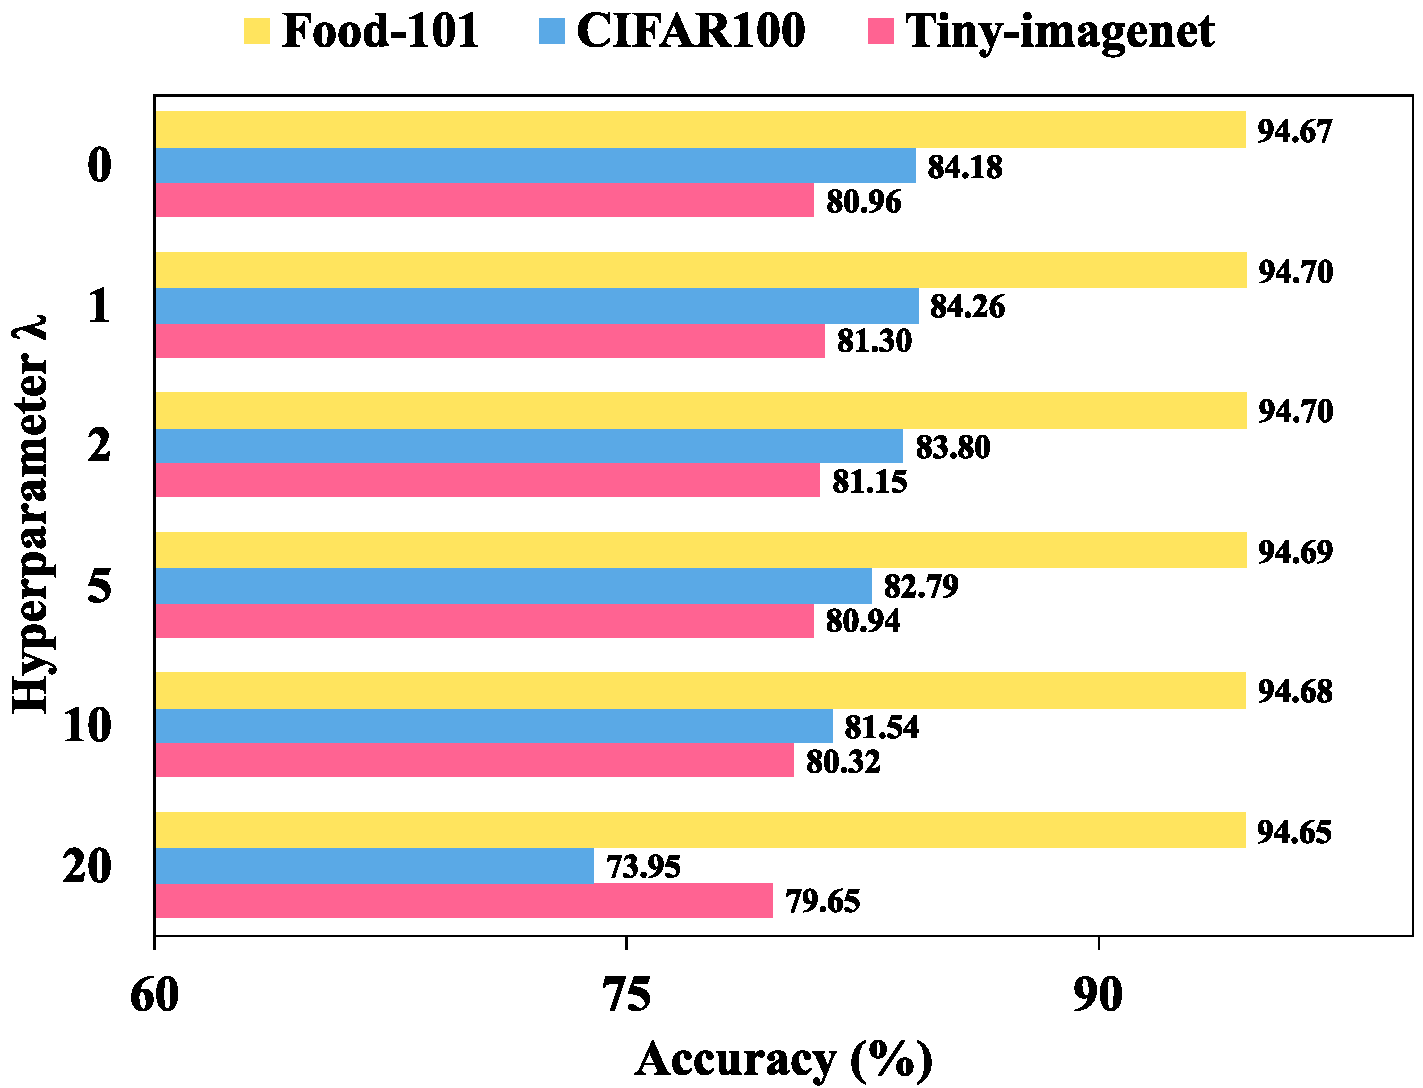
\includegraphics[width=\linewidth]{./Figures/lam.pdf}
  \caption{Experimental results on the influence of the consistency weight hyperparameter $\lambda$ using FCL-C data.}
  \label{fig:lam}
\end{figure}

\subsection{Results of FCL-C}
Table~\ref{tab:method-compare-clip} compares FCL with the weakly supervised baselines on five benchmarks and includes FSL-C as a fully supervised reference.

FCL achieves higher accuracy than the compared weakly supervised baselines on all five datasets. On EuroSAT, the gain over the strongest weakly supervised baseline in Table~\ref{tab:method-compare-clip} is $12.77$ percentage points; the gain over the additional FixMatch-style control is $3.33$ points. FCL also approaches the fully supervised reference on several datasets while correcting only a subset of training labels.

\begin{figure}[t]
  \centering
  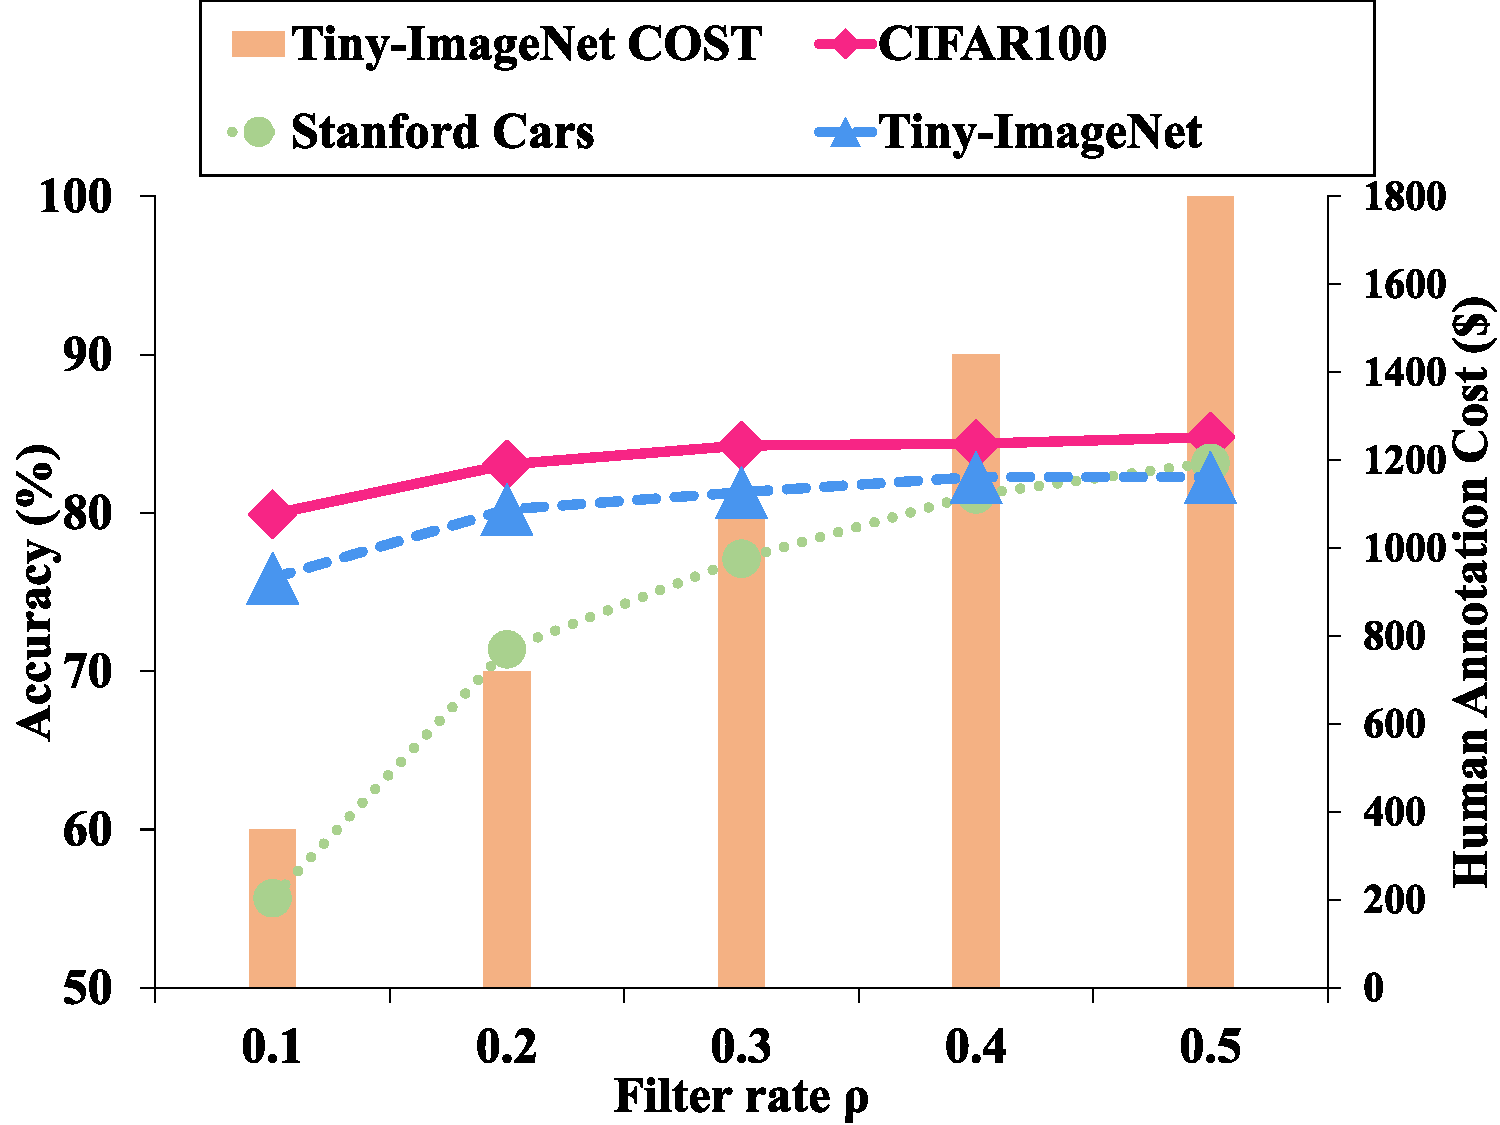
\includegraphics[width=0.9\linewidth]{./Figures/rho2.pdf}
  \caption{Classification accuracy versus correction rate on Tiny-ImageNet. The cost axis is a linear query-count proxy under a fixed per-image price assumption, rather than measured human annotation expenditure.}
  \label{fig:rho}
\end{figure}


\subsection{Selection and Loss Controls}
The supplementary controls separate two design choices. Replacing random selection with prototype selection under CE increases accuracy by $0.11$--$3.08$ percentage points across the five datasets. With the prototype filter retained, FCL exceeds mixed-label CE by $2.07$--$35.03$ points. Table~\ref{tab:component-controls} brings these existing controls together. These comparisons motivate the selection and ranking components, but isolating their interaction also requires a random-selection version of AUC-C and matched sampling and learning-rate schedules.

\begin{table*}[t]
\caption{Existing selection and loss controls, reported as test accuracy (\%). Both CE controls use mixed corrected and uncorrected hard targets. FCL uses CE on corrected samples and AUC-C on uncorrected samples. These controls do not by themselves isolate differences in sampling or optimization.}
\label{tab:component-controls}



\centering
\small
\begin{tabular*}{\textwidth}{@{\extracolsep{\fill}}lrrrrr}
\toprule
Method & CIFAR-100 & Caltech-101 & EuroSAT & Food-101 & Tiny-ImageNet \\
\midrule
Random-Filter-CE & 80.78 & 89.29 & 55.33 & 91.22 & 81.21 \\
FCL-Filter-CE & 81.94 & 89.40 & 58.41 & 91.75 & 82.16 \\
FCL (ours) & 85.02 & 96.20 & 93.44 & 94.78 & 84.23 \\
\bottomrule
\end{tabular*}

\end{table*}

\subsection{Influence of Hyperparameter \texorpdfstring{$\lambda$}{lambda}}
We examine $\lambda$, which balances corrected-sample cross-entropy and AUC-C, on CIFAR-100, Food-101, and Tiny-ImageNet while fixing all other training settings.

At $\lambda=0$, FCL uses only corrected-sample cross-entropy but retains class-balanced sampling and its learning-rate schedule. FL-C in Table~\ref{tab:method-compare-clip} instead uses shuffled corrected-only batches and a fixed learning rate. Their shared loss therefore does not imply identical accuracy.

Accuracy improves as $\lambda$ increases from $0$ to $1$, peaks near $1$, and then declines. Small $\lambda$ underuses uncorrected samples, whereas large $\lambda$ overemphasizes potentially noisy pairwise comparisons. The sharp decline on CIFAR-100 from $\lambda=10$ to $20$ suggests greater sensitivity to excessive AUC-C weighting.


\subsection{Impact of \texorpdfstring{$\rho$}{rho} and Human Annotation Cost}
To investigate the effect of the filter rate $\rho$, we conducted a controlled experiment to analyze how varying the proportion of filtered area influences the overall precision of the classification. The filter rate $\rho$ determines the percentage of instances that need to be corrected, measured by the distance of cosine from the class prototype, that are selected for human correction. 

As shown in Figure~\ref{fig:rho}, the overall classification accuracy increases steadily as the filter rate $\rho$ increases. A larger $\rho$ introduces a greater proportion of human-corrected samples into the training set, thereby reducing the influence of noisy labels in the uncorrected subset. The number of training-label queries is approximately $N\rho$. Under a constant per-query cost $C_h$, the corresponding proxy is $C(\rho)=N\rho C_h$. This model excludes labeled validation data, feature extraction, model inference, and differences in the time required to correct individual images; no human timing study is conducted.

We observe that the accuracy curve begins to enter a plateau phase after $\rho=0.3$, where further increasing human correction yields diminishing marginal returns in precision. At $\rho=0.3$, the nominal number of queried training labels is $70\%$ lower than labeling every training image. We use this rate as the default operating point; the experiment does not establish a universally optimal correction budget.

\begin{table}[!t]
\caption{Classification accuracy (\%) under simulated errors in the corrected labels on four datasets. Column headers indicate the proportion of correct labels within the corrected subset, with the filter rate fixed at $\rho=0.3$.}
\label{tab:human-correction-noise}



\centering
\small
\setlength{\tabcolsep}{3pt}
\begin{tabular*}{\columnwidth}{@{\extracolsep{\fill}}lccccc}
\toprule
Dataset & $100\%$ & $95\%$ & $90\%$ & $85\%$ & $80\%$ \\
\midrule
CIFAR-100     & 85.02 & 83.65 & 83.17 & 82.78 & 82.39 \\
Caltech-101   & 96.20 & 95.76 & 95.71 & 95.27 & 94.91 \\
EuroSAT       & 93.44 & 89.69 & 87.54 & 85.69 & 83.53 \\
Tiny-ImageNet & 84.23 & 83.30 & 82.52 & 82.07 & 81.44 \\
\bottomrule
\end{tabular*}

\end{table}



% EXP E3: synthetic correction-noise study is retained; add seeds and matched baselines for robustness claims.
\subsection{Impact of Synthetic Correction Errors}
To evaluate sensitivity to simulated correction errors, we vary correction accuracy from $100\%$ to $80\%$ in steps of $5\%$ by replacing selected corrected labels with uniformly sampled incorrect classes. The feature cache, data partitions, prototype filter, and uncorrected annotations remain fixed, with $\rho=0.3$. All other experimental settings follow the main experiments.

As shown in Table~\ref{tab:human-correction-noise}, at $95\%$ correction accuracy, the decrease relative to the $100\%$ reference is below one percentage point on two datasets, while CIFAR-100 and EuroSAT lose $1.37$ and $3.75$ percentage points, respectively. At $80\%$, the decrease ranges from $1.29$ percentage points on Caltech-101 to $9.91$ percentage points on EuroSAT. Accuracy decreases consistently as correction errors increase across all four datasets. These results indicate tolerance to modest correction errors on several datasets, while the larger decline on EuroSAT highlights the importance of reliable corrected labels for FCL with AUC-C.

\section{Conclusion}
In this paper, we study Filter-Corrected Labels (FCL-C), which is a prototype-based filtering and correction mechanism to improve the reliability of noisy labels generated by VLMs. Furthermore, we introduce an AUC-based consistency objective that operates exclusively on the uncorrected data to stabilize pairwise rankings.
Experiments on five benchmarks show improved accuracy over the compared implementations. Additional controls examine selection, loss design, four frozen CLIP encoders on EuroSAT, and simulated correction errors. The evidence is limited to frozen-feature classification, single-seed results, and simulated correction; measured human effort and broader deployment remain to be evaluated.

\section*{LLM Usage Statement}
OpenAI Codex was used to assist with manuscript editing, mathematical notation checks, and literature search. CLIP was used to generate pseudo-labels and class scores as described in the method. No new experiments or experimental measurements were generated during the manuscript revision.

{
    \small
    \bibliographystyle{ieeenat_fullname}
    \bibliography{main}
}

% WARNING: do not forget to delete the supplementary pages from your submission 
% \clearpage
\setcounter{page}{1}
\maketitlesupplementary


\section{Rationale}
\label{sec:rationale}
% 
Having the supplementary compiled together with the main paper means that:
% 
\begin{itemize}
\item The supplementary can back-reference sections of the main paper, for example, we can refer to \cref{sec:intro};
\item The main paper can forward reference sub-sections within the supplementary explicitly (e.g. referring to a particular experiment); 
\item When submitted to arXiv, the supplementary will already included at the end of the paper.
\end{itemize}
% 
To split the supplementary pages from the main paper, you can use \href{https://support.apple.com/en-ca/guide/preview/prvw11793/mac#:~:text=Delete%20a%20page%20from%20a,or%20choose%20Edit%20%3E%20Delete).}{Preview (on macOS)}, \href{https://www.adobe.com/acrobat/how-to/delete-pages-from-pdf.html#:~:text=Choose%20%E2%80%9CTools%E2%80%9D%20%3E%20%E2%80%9COrganize,or%20pages%20from%20the%20file.}{Adobe Acrobat} (on all OSs), as well as \href{https://superuser.com/questions/517986/is-it-possible-to-delete-some-pages-of-a-pdf-document}{command line tools}.

\end{document}
